\documentclass[tikz,border=5pt]{standalone}
\usepackage{pgfplots}\pgfplotsset{compat=1.18}
\definecolor{tramU}{HTML}{365FB3}\definecolor{tramDos}{HTML}{0F766E}\definecolor{punt}{HTML}{B91C1C}
\begin{document}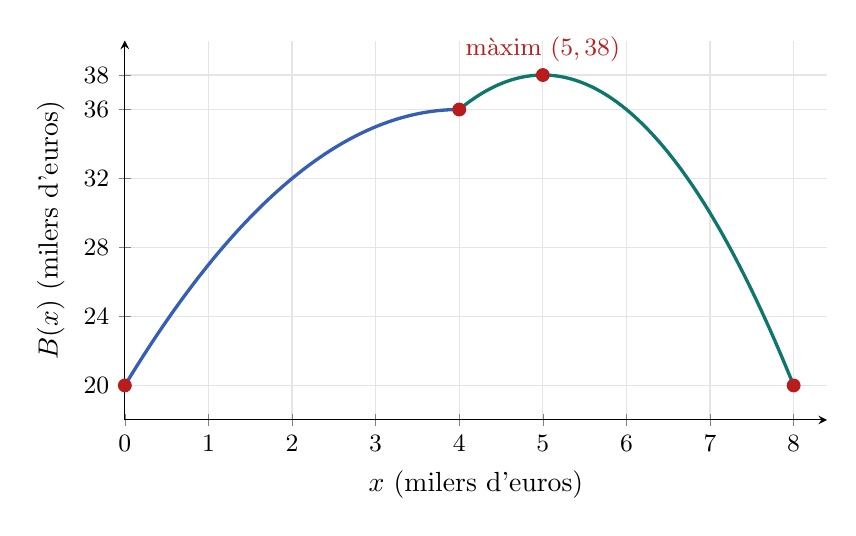
\begin{tikzpicture}
\begin{axis}[width=10.5cm,height=6.4cm,axis lines=left,xmin=0,xmax=8.4,ymin=18,ymax=40,
 xlabel={$x$ (milers d'euros)},ylabel={$B(x)$ (milers d'euros)},grid=major,grid style={black!10},
 xtick={0,1,...,8},ytick={20,24,28,32,36,38},tick label style={font=\small},clip=false]
 \addplot[tramU,very thick,domain=0:4,samples=120]{-x^2+8*x+20};\addplot[tramDos,very thick,domain=4:8,samples=120]{-2*x^2+20*x-12};
 \addplot[only marks,mark=*,mark size=2.3pt,punt] coordinates {(0,20)(4,36)(5,38)(8,20)};
 \node[anchor=south,font=\small,text=punt] at (axis cs:5,38.2) {màxim $(5,38)$};
\end{axis}\end{tikzpicture}\end{document}
